{\bfseries Производственные и обрабатывающие отрасли}

{\bfseries МРНТИ: 52.13.17; 20.51.23; 87.15.15; 44.01.75}

\begin{quote}
{\bfseries НАПРАВЛЕНИЯ ПОВЫШЕНИЯ ЭНЕРГОЭФФЕКТИВНОСТИ НА ОТКРЫТЫХ
РАЗРАБОТКАХ МЕСТОРОЖДЕНИЙ ПОЛЕЗНЫХ ИСКОПАЕМЫХ}
\end{quote}

{\bfseries С.Ж. Галиев\textsuperscript{1*}, Е.Т.Утешов\textsuperscript{1*},
Д.А. Галиев\textsuperscript{1}, Ж.С. Бексапин \textsuperscript{2}}

Институт горного дела им. Д.А.Кунаева РГП «НЦ КПМС» МИИР РК, г. Алматы,
Казахстан,

ТОО «Qazakstan smart technology», г. Алматы, Казахстан,

email: seitgaligaliyev@mail.ru

Статья посвящена актуальной теме, в которой сочетаются проблемные
вопросы энергоэффективности и низкоуглеродного развития горного
производства. В ней раскрываются подходы и методические аспекты анализа
и оценки энергоэффективности горных предприятий с открытым способом
освоения месторождений твёрдых полезных ископаемых. В основе методологии
лежит процессный подход, базирующийся на процессах цифровизации,
развития информационных технологий и соответствующего
программно-методического обеспечения с применением эффективного для
решения данного рода задач метода имитационного моделирования. В статье
раскрываются результаты проведения комплексных технико-технологических и
энерго- аудитов, позволяющих выявлять реальный потенциал повышения
энергоэффективности и направления его реализации с последующей
выработкой комплекса конкретных мер в данном направлении. Одними из
основных выводов является вывод о наличии существенно потенциала
повышения энергоэффективности (10-15\%) и обоснование необходимости
формирования на горных предприятиях автоматизированных систем энерго- и
экологического мониторинга, позволяющих, с одной стороны, своевременно и
целенаправленно вырабатывать оперативные управленческие меры, а с
другой, повысить эффективность реализации принципа экологичности и
безопасности в процессе технологической модернизации горных производств.

{\bfseries Ключевые слова:} Открытые горные работы, геотехнологический
комплекс,

экологические выбросы, энергоэффективность, энергосбережение, экономика,
оптимизация, автоматизация.

{\bfseries ПАЙДАЛЫ ҚАЗБАЛАР КЕН ОРЫНДАРЫН АШЫҚ ИГЕРУДЕГІ ЭНЕРГИЯ
ТИІМДІЛІГІН АРТТЫРАУ БАҒЫТТАРЫ}

{\bfseries С.Ж. Ғалиев\textsuperscript{1*}, Е.Т. Өтешов\textsuperscript{1},
Д.А. Ғалиев\textsuperscript{1}, Ж. С. Бексапин\textsuperscript{2}}

Д. А. Қонаев атындағы Тау-кен институты. Д. А. Қонаева ҚР ИИДМ

"КПМС ҰО" РМК, Алматы қ., Қазақстан, "Qazakstan smart technology" ЖШС,
Алматы қ., Қазақстан,
е-mail:~\href{https://e.mail.ru/compose/?mailto=mailto\%3aseitgaligaliyev@mail.ru}{seitgaligaliyev@mail.ru}~

Мақала энергия тиімділігі мен тау-кен өндірісінің төмен көміртекті
дамуының проблемалық мәселелерін біріктіретін өзекті тақырыпқа арналған.
Онда қатты пайдалы қазбалар кен орындарын игерудің ашық тәсілімен
тау-кен кәсіпорындарының энергия тиімділігін талдау мен бағалаудың
тәсілдері мен әдістемелік аспектілері ашылады. Әдістеме цифрландыру,
ақпараттық технологияларды дамыту және осы типтегі міндеттерді шешуде
тиімді модельдеу әдісін қолдана отырып, тиісті бағдарламалық-әдістемелік
қамтамасыз ету процестеріне негізделген процестік тәсілге негізделген.
Мақалада энергия тиімділігін арттырудың нақты әлеуетін және оны іске
асыру бағытын анықтауға мүмкіндік беретін кешенді
техникалық-технологиялық және энергетикалық аудиттерді жүргізу
нәтижелері, содан кейін осы бағытта нақты шаралар кешені әзірленеді.
Негізгі тұжырымдардың бірі-энергия тиімділігін арттырудың айтарлықтай
әлеуетінің болуы туралы қорытынды (10-15\%) және негіздеме.

{\bfseries Түйінді сөздер:} Ашық тау-кен жұмыстары, геотехнологиялық кешен,
экологиялық шығарындылар, энергия тиімділігі, энергия үнемдеу,
экономика, оңтайландыру, автоматтандыру.

{\bfseries DIRECTIONS OF ENERGY EFFICIENCY IMPROVEMENT IN OPEN PIT MINING
OF MINERAL DEPOSITS}

{\bfseries S.Zh. Galiev\textsuperscript{1*}, E.T.
Uteshov\textsuperscript{1}, D.A. Galiev\textsuperscript{1},Zh.S
Beksapin\textsuperscript{2}}

Mining Institute after D.A. Kunayev of RSE "NC KPMC" MIIR RK, Almaty,
Kazakhstan, Almaty, Kazakhstan, Qazakstan smart technology" LLP, Almaty,
Kazakhstan,

е-mail:~\href{https://e.mail.ru/compose/?mailto=mailto\%3aseitgaligaliyev@mail.ru}{seitgaligaliyev@mail.ru}~

The article is devoted to the actual topic, which combines the
problematic issues of energy efficiency and low-carbon development of
mining production. It reveals the approaches and methodological aspects
of the analysis and assessment of energy efficiency of mining
enterprises with the open-pit method of development of deposits of solid
minerals. The methodology is based on the process approach based on the
processes of digitalization, development of information technologies and
corresponding software and methodological support with the use of
simulation modeling method effective for solving this kind of problems.
The article reveals the results of comprehensive technical and
technological and energy audits, which allow to identify the real
potential of energy efficiency and areas of its implementation with the
subsequent development of a set of specific measures in this direction.
One of the main conclusions is the conclusion that there is a
significant potential to increase energy efficiency (10-15\%) and the
rationale for the need to form automated energy and environmental
monitoring systems at mining enterprises, allowing, on the one hand,
timely and targeted development of operational management measures, and
on the other hand, to improve the effectiveness of the principle of
environmental and safety in the process of technological modernization
of mining production.

{\bfseries Keywords:} open-pit mining, geotechnological complex,
environmental emissions, energy efficiency, energy conservation,
economy, optimization, automation.

{\bfseries Введение.} Вопросы энергоэффективности традиционно имеют высокую
актуальность, которая в последние десятилетия усиливается проблемами
экологии и глобального потепления. Эти вопросы становятся центральной
темой ежегодных глобальных форумов, проходящих с участием
правительственных делегаций стран мира. Казахстан в этом плане
присоединился к международным инициативам приняв Указом Президента
Республики Казахстан от 2 февраля 2023 года за № 121 Стратегию
достижения углеродной нейтральности Республики Казахстан до 2060 года.
Для Казахстана проблема энергоэффективности актуальна и в связи с тем,
что основным источником энергии в стране является уголь. Практически всё
промышленное производство страны подпадает под экологические санкции,
выдвигаемые международным сообществом, и проблема снижения экологических
выбросов жёстко коррелирует с задачами повышения энергоэффективности.
Особенно жёстко данный вопрос стоит перед горнодобывающей отраслью
экономики, являющейся одной из самых энергозатратных, а также и одним из
крупнейших загрязнителей окружающей среды.

По результатам ряда проведённых исследований, очевиден существенный
потенциал повышения энергоэффективности, реализация которого сопряжена
со снижением себестоимости горнотранспортных работ в среднем на 10-15\%.
Для Казахстана это принципиально важно не только по экономическим
аспектам, но также в связи с повышением рентабельности освоения
отечественной минерально-сырьевой базы и выполнением принятых
международных обязательств о снижении выбросов к 2030 г. на 15\%
относительно уровня выбросов 1990 г. (безусловная цель) и доведение
сокращения на 25 \% при условии получения международной поддержки на
декарбонизацию экономики (условная цель) {[}1{]}.

Для Казахстана достижение углеродной нейтральности является достаточно
амбициозной задачей, которую планируется достичь через реализацию
инициатив по трем ключевым направлениям, одно из которых -
декарбонизация отраслей и процессов, связанных с ископаемым топливом
{[}2{]}. При этом, выбросы парниковые газы, связанные с ископаемым
топливом, будут сокращены посредством перехода от использования
ископаемого топлива и его производных к альтернативным и возобновляемым
источникам энергии, путём повышения энергоэффективности и
энергосбережения, взятием курса на дальнейшую электрификацию (замещения
установок, сжигающих топливо, на технологии, работающие на основе
электроэнергии).

\emph{Потенциал повышения энергоэффективности и достижения углеродной
нейтральности в горнодобывающей отрасли Казахстана:}

По данным казахстанской статистики на современном этапе 86,6\% выбросов
в РК приходится на промышленность, в т.ч. на горнодобывающую - 53,45\%
(11, 2 млн. тонн в год). Энергоемкость продукции ГМК превышает
аналогичный показатель ОЭСР более чем в 2 раза. Наибольшие выбросы и
расход топлива приходятся на автотранспорт. В общем объеме
производственных затрат ГМК, расходы на дизельное топливо и
электроэнергию составляют около 50\%.

Если проанализировать возможные направления повышения
энергоэффективности и снижения углеродоёмкости горного производства, то
их можно сформулировать следующим образом:

- за счёт оптимизации производственных и технологических процессов --
потенциал до 15\% с достижением экономических эффектов в виде снижения
себестоимости горнотранспортных работ до 10-15\%/год при попутном
повышении технологической культуры;

- перевод автотранспорта на газодизельные двигатели -- снижение до
25-30\% экологических выбросов, сопровождающееся аналогичным где-то
снижением себестоимости горнотранспортных работ;

- адаптация транспортной инфраструктуры и структуры энергосетей со
структурой минерально-сырьевой базы Республики Казахстан -- потенциал
снижения объёмов выбросов СО2 и снижения себестоимости около 5-10\%;

- разработка технологий снижения (декарбонизация) выбросов загрязняющих
веществ (УХУ: улавливание до 90\%, хранение и утилизация -- до 100\%);

- совершенствование технологий в рамках процесса технологической
модернизации -- долгосрочная перспектива с потенциалом до 100\%
(экскаваторно-конвейерные комплексы, скиповые подъёмники и др.);

- освоение технологий подземного скважинного выщелачивания (ПСВ) для
освоения месторождений руд цветных и чёрных металлов -- до 100\%;

- комплексное освоение минерально-сырьевой базы Казахстана -- помимо
значительного снижения углеродоёмкости, снижение затрат на извлечение
сокращается в разы;

- перевод системы энергообеспечения ГМК РК на альтернативные и
возобновляемые источники (водород, солнечная и ветряная энергия, водные
электростанции, урановое производство и атомные электростанции) -- до
100\% снижение углеродоёмкости;

- разработка нанотехнологий освоения месторождений полезных ископаемых
-- касается практически всей минерально-сырьевой базы -- потенциал до
100\%.

В приведенном перечне, первые два направления могут быть
первоочередными, так как не требуют каких-либо особых дополнительных
вливаний. Тут достаточно поддержки развития программно-методического
обеспечения на основе пооперационной цифровизации и углубленной
аналитики в рамках широко применяемых сегодня инструментов
финансирования науки. С этой целью необходимо привлечение таких
инструментов инновационно-индустриального развития и стимулирования
технологической модернизации, как проведение комплексных
технико-технологических аудитов и совершенствование энергоаудитов, что
позволит своевременно и точно определять имеющийся потенциал,
направления и меры по его своевременной реализации.

{\bfseries Материалы и методы - методология оценки энергоэффективности.}
Комплексный технико-технологический аудит проектных решений по
формированию, а также эксплуатируемых геотехнологических комплексов
осуществляется на основе системного подхода, при котором одним из
ключевых факторов является адекватный учёт процессности в управлении
горнотранспортными работами. В свою очередь, этот подход основывается и
реализуется в рамках теории и методологии модернизации, индустриализации
и технологической модернизации {[}3-4{]}.

Рассматриваемый подход предполагает использование наиболее эффективного
на данном направлении метода имитационного логико-статистического
моделирования, обеспечивающего достоверное воспроизведение порядка и
последовательности основных технологических и
организационно-экономических операций в конкретных горнотехнических,
горно-геологических, горно-геометрических, организационных и
экономических условиях. В настоящее время данные подход и метод уже боле
40 лет широко применяются для технико-экономического анализа
эффективности функционирования геотехнологических комплексов на открытых
разработках с использованием цикличных технологий с автомобильным,
железнодорожным и комбинированным автомобильно-железнодорожным видами
транспорта горной массы.

Основной целью комплексного технико-технологического аудита является
оценка эффективности, включая энергоэффективность, функционирования
геотехнологического комплекса, выявление имеющегося потенциала,
направлений и установления мер по его реализации.

В случае рассмотрения геотехнологического комплекса с применением
автотранспорта, основными элементами его, как системы, являются
карьерная автотрасса, экскаваторный и автомобильный парки, геометрия
карьерного пространства, принятые на предприятии организационные меры и
нормативы. По автотрассе адекватно учитываются её структура со всеми
технологическими особенностями и фактического расположения блок-участков
в карьерном пространстве, их геометрия (уклон, протяжённость,
криволинейность) и качество применяемого дорожного покрытия, а также
затраты на их формирование и поддержание в рабочем состоянии. По
экскаваторному и автомобильному парку достоверному учёту подлежат
основные паспортные технико-технологические характеристики (ёмкость
кузова и ковша, КПД трансмиссии и двигателей, их мощностные
характеристики, сроки эксплуатации и принятые нормативы по
эксплуатации), модели и число работающего и списочного парков, а также
их стоимостные характеристики (остаточная стоимость, цены, нормы
амортизации). Параметры принципиальных характеристик карьерного
пространства учитываются благодаря использованию графических документов,
полученных с использованием специализированной программы AutoCAD.

Одним из важнейших направлений комплексного технико-технологического
аудита является оценка его энергоэффективности. Энергоёмкость основных
технологических процессов при освоении месторождений твёрдых полезных
ископаемых открытым способом и с применением цикличных технологий добычи
занимает в среднем 60-70 \% в общей себестоимости горнотранспортных
работ. При заданных технологиях освоения месторождений, когда определены
направления и порядок ведения добычных и вскрышных работ, основные
направления поиска потенциала снижения энергоёмкости технологических
связаны с соответствующим выбором моделей основного горного и
транспортного оборудования, режимом и условиями их эксплуатации
{[}5-11{]}.

В свою очередь, исследование режимов эксплуатации основного горного и
транспортного оборудования требует соответствующих методов и подходов,
позволяющих вести адекватный учёт основных влияющих на результативность
работы горнотранспортного комплекса факторов, как это показано на
рисунке 1. Это позволяет оценивать энергоэффективность исходя из
адекватного учёта пооперационного расхода энергии и характера интеграции
этих долей энергии в формирующиеся энергопотоки технологического
процесса в целом.

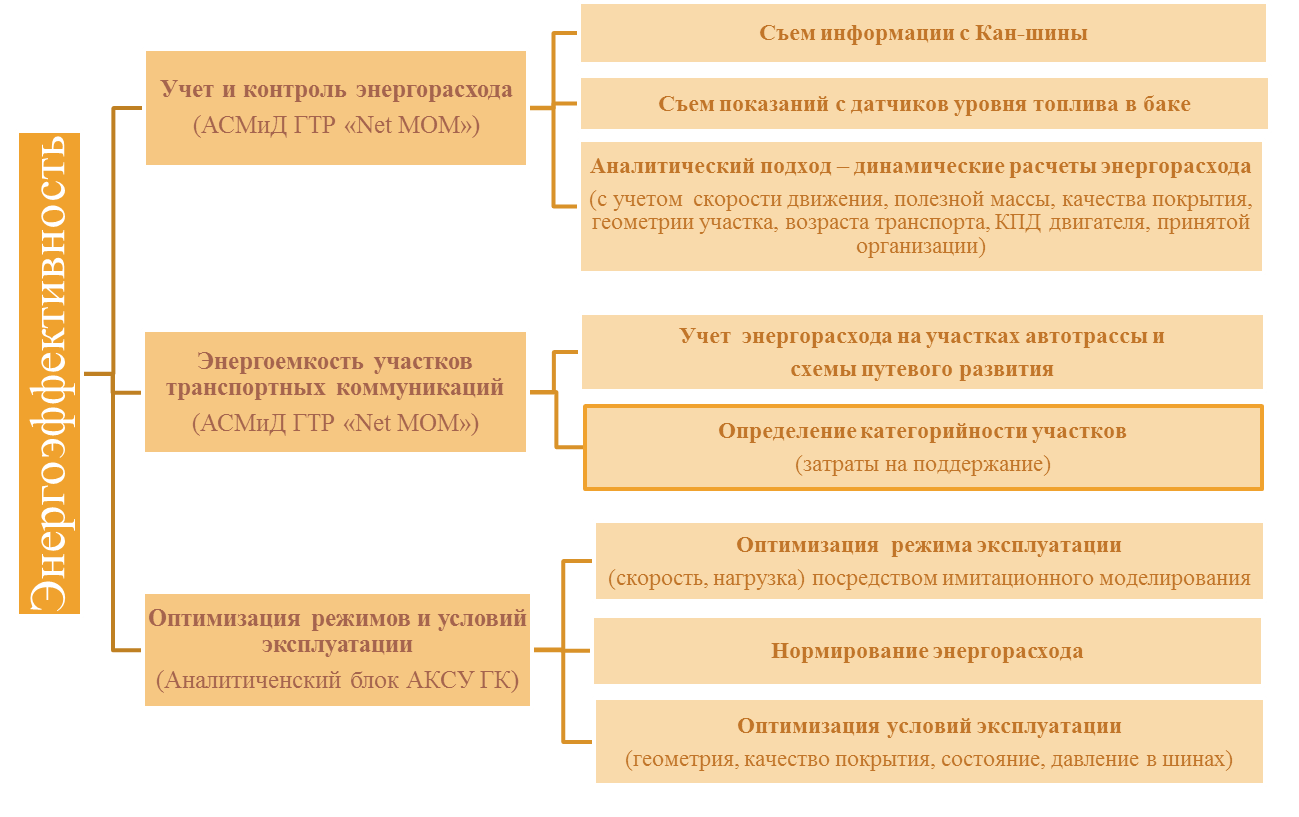
\includegraphics[width=0.8\textwidth]{image48}

Рис. 1 -- Концепция энергосбережения на открытых разработках

Энергоэффективность предполагает не только простое снижение
энергорасхода, а прежде всего в увязке с общей эффективностью
функционирования геотехнологического комплекса, которая оценивается с
применением комплекса технико-экономических критериев. В связи с этим,
принципиально важным в процессе анализа и оценки энергоэффективности
исследуемых технологических процессов основываться на адекватном учёте
пооперационных затрат горнотранспортного процесса и технического
состояния машин. Одним из принципиальных показателей в этом плане
является КПД двигателя автосамосвала, который имеет зависимость своего
значения от возраста эксплуатируемых машин (см. рис.2). Это позволяет
достоверно оценивать экономическую эффективность энергорасхода,
способность энергии к обеспечению повышенной производительности, а,
следовательно, устанавливать уровень его целесообразности. Для этих
целей применяется методология экономики процессного управления.

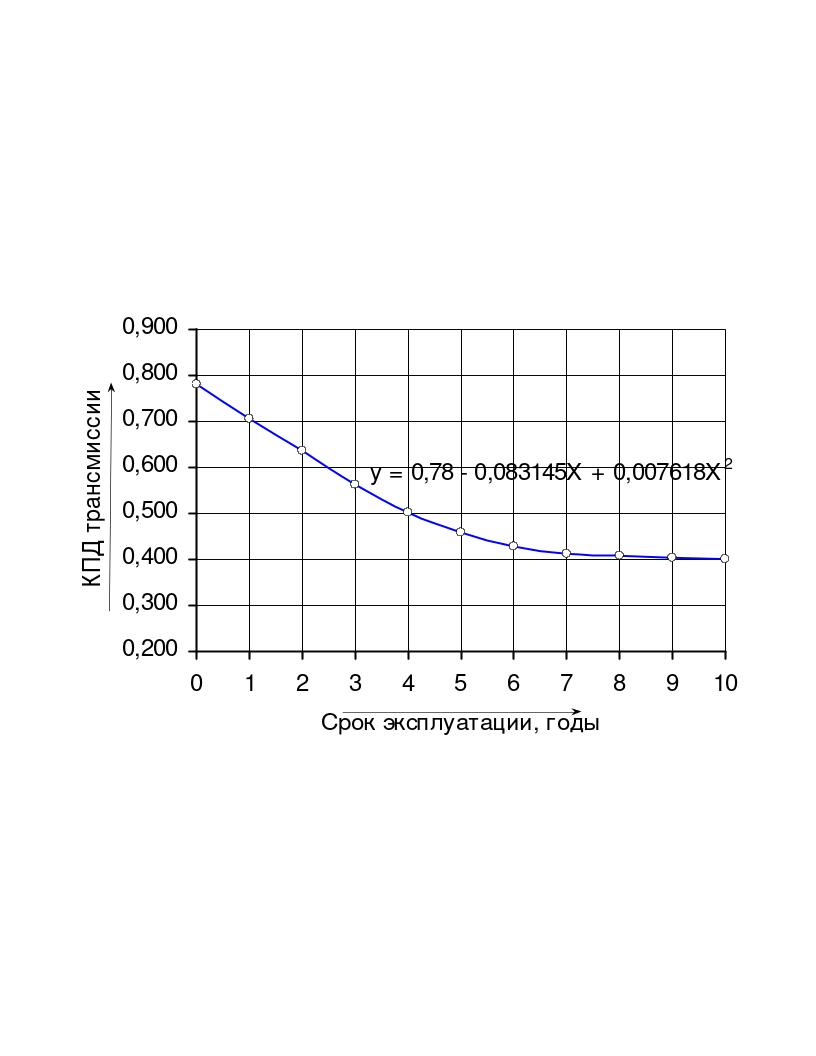
\includegraphics[width=0.8\textwidth]{image49}

Рис. 2 - Зависимость КПД двигателя автосамосвала от срока эксплуатации

Другим важным моментом в применяемом подходе является адекватный
динамический подход к учёту энергорасхода автосамосвалами в зависимости
от паспортных тяговых характеристик двигателей и трансмиссии машин (см.
рисунок 3), позволяющих воспроизводить реальную процессную взаимосвязь в
динамике скорости движения автосамосвала и энергорасхода в зависимости
от режима и условий их эксплуатации -- качества дорожного покрытия,
геометрия по участкам автотрассы, техническое состояние и режим загрузки
автосамосвалов (вровень, «с шапкой», «без шапки»).

По специализированным карьерным автосамосвалам тяговые характеристики
являются паспортными, полученные заводом изготовителем, а по
автосамосвалам не специализированным они были получены путём перевода из
имеющейся формы отражения тяговых характеристик (часто в место тяговых
усилий указываются обороты двигателя). Данный способ учёта энергорасхода
является наиболее достоверным и обеспечивает адекватную чувствительность
к изменениям всех обозначенных принципиальных факторов, обуславливающих
энергорасход. Тяговые характеристики вшиты в модели автосамосвалов и
своевременно используются алгоритмом в процессе моделирования.

По погрузочному оборудованию, учёт энергорасхода (электричество,
дизельное топливо) осуществляется в зависимости от КПД двигателя,
времени циклов, ёмкости ковша и плотности экскавируемых горных пород с
учётом соответствующего коэффициента разрыхления.

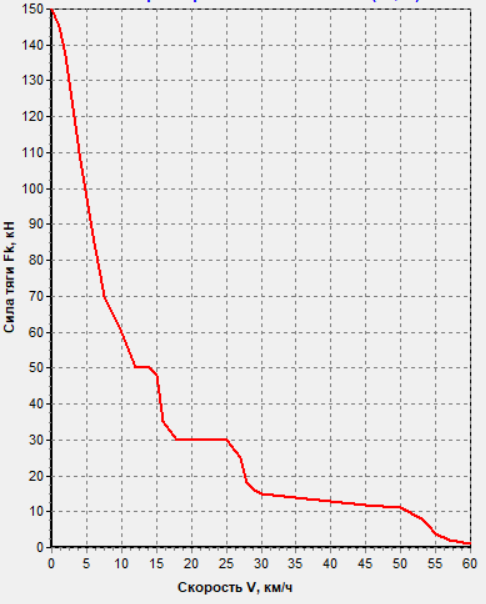
\includegraphics[width=0.8\textwidth]{image50}

Рис. 3. - Тяговые характеристики автосамосвалов БелАЗ-7540

Для адекватного учёта энергорасходов на участках транспортных
коммуникаций необходимо достоверное воспроизведение их структуры и
характеристик качественных и технологических, как это показано на
рисунке 4. С этой целью используется план (фактический или проект)
горных работ, выполненный в AutoCAD либо полученный с использованием
широко ныне используемых летательных аппаратов дронов, которые позволяют
с максимальной точностью воспроизводить на имитационных цифровых моделях
в трёхмерном пространстве горно-геометрические параметры. С планов
горных работ и из пояснительных записок по ним берутся необходимые
организационные и технико-технологические характеристики по ним. Это
позволяет точно позиционировать в карьерном пространстве все имеющиеся
пункты погрузки-выгрузки и перегрузки горной массы, а следовательно,
адекватно учитывать структуры формируемых рудо- и породо- потоков.

Таким образом, проведение комплекса исследований предполагается на
основе системного подхода с применением методологии имитационного
моделирования исследуемых горнотранспортных процессов, обеспечивающих
адекватный учёт порядка и последовательности операций основных
технологических процессов с достоверным учётом конкретных
горнотехнических, горно-геометрических, горно-геологических,
организационных и экономических условий функционирования основного
технологического комплекса разрезов {[}6-10{]}.

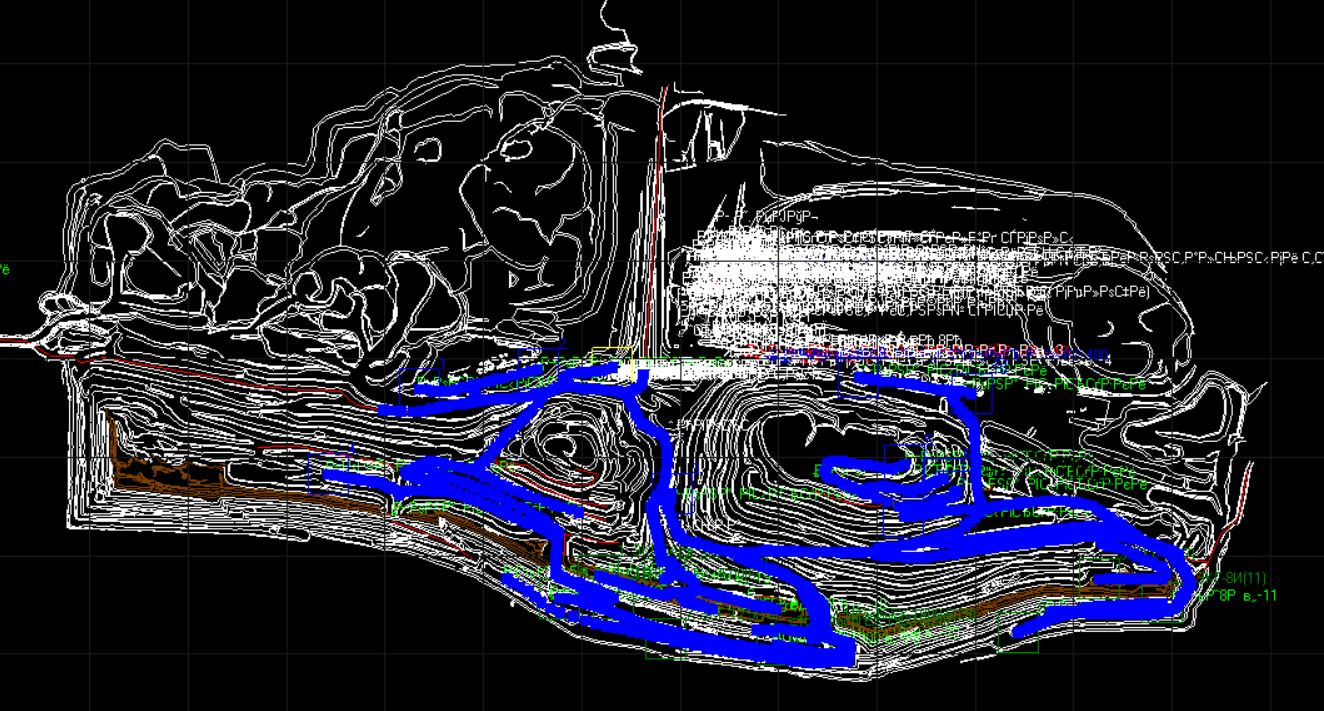
\includegraphics[width=0.8\textwidth]{image51}

Рис. 4 - План разреза «Центральный» с встроенной структурой модели
горнотранспортного комплекса

Применяемая в процессе имитационного моделирования и исследований
методология формирования экономико-математических моделей обеспечивает
адекватный учёт порядка и последовательности пооперационных затрат на
поддержание работы горнотранспортного комплекса.

Одно из достоинств применяемого подхода заключается в практически
достоверном учёте общего режима и календаря эксплуатации
горнотранспортных комплексов разрезов, что имеет принципиальное значение
для обеспечения точности основных технико-экономических расчётов и
эффективности комплекса предлагаемых мер.

{\bfseries Результаты и обсуждение -} направления повышения эффективности.

Возможные в рамках данного направления повышения энергоэффективности под
направления можно увидеть по таблице 1, где на примере одного из
исследуемых объектов, среди с общепроизводственных мероприятий,
наибольшую долю (до 90\%) имеющегося потенциала имеют улучшение качества
покрытия внутрикарьерных дорог, внедрение автоматизированной системы
мониторинга энергорасхода, и оптимизации парка автосамосвалов, а также
режимов и условий их эксплуатации.

Таблица 1. План энергосберегающих мероприятий по предприятию

\begin{longtable}[]{@{}
  >{\raggedright\arraybackslash}p{(\columnwidth - 8\tabcolsep) * \real{0.0551}}
  >{\raggedright\arraybackslash}p{(\columnwidth - 8\tabcolsep) * \real{0.4444}}
  >{\raggedright\arraybackslash}p{(\columnwidth - 8\tabcolsep) * \real{0.1213}}
  >{\raggedright\arraybackslash}p{(\columnwidth - 8\tabcolsep) * \real{0.1820}}
  >{\raggedright\arraybackslash}p{(\columnwidth - 8\tabcolsep) * \real{0.1972}}@{}}
\toprule\noalign{}
\multirow{2}{*}{\begin{minipage}[b]{\linewidth}\raggedright
{\bfseries № п/п}
\end{minipage}} &
\multirow{2}{*}{\begin{minipage}[b]{\linewidth}\raggedright
{\bfseries Наименование мероприятий}
\end{minipage}} &
\multirow{2}{*}{\begin{minipage}[b]{\linewidth}\raggedright
{\bfseries Затраты, тыс. тенге}
\end{minipage}} &
\multicolumn{2}{>{\raggedright\arraybackslash}p{(\columnwidth - 8\tabcolsep) * \real{0.3792} + 2\tabcolsep}@{}}{%
\begin{minipage}[b]{\linewidth}\raggedright
{\bfseries Годовая экономия топливно-энергетических ресурсов}
\end{minipage}} \\
& & & \begin{minipage}[b]{\linewidth}\raggedright
в натуральном выражении, т.у.т.
\end{minipage} & \begin{minipage}[b]{\linewidth}\raggedright
в стоимостном выражении, тыс. тенге
\end{minipage} \\
\midrule\noalign{}
\endhead
\bottomrule\noalign{}
\endlastfoot
{\bfseries 1} & Замена деревянных окон на металлопластиковые,
энергосберегающие окна & 86954 & 114,17 & 539,52 \\
{\bfseries 2} & Установка ПВХ завес на воротах & 5401,1 & 319,27 &
1508,69 \\
{\bfseries 3} & Применение низкоэмиссионных пленок на окнах & 16210,9 &
219,62 & 889,72 \\
{\bfseries 4} & Установка теплоотражающих экранов на стенах за приборами
отопления & 228,78 & 11,37 & 53,74 \\
{\bfseries 5} & Замена неизолированного провода типа А и АС ВЛ 0,4 кВ на
провод типа СИП & 35811,43 & 30,37 & 6557,7 \\
{\bfseries 6} & Замена устаревших трансформаторов типа ТМ на
энергоэффективные трансформаторы типа ТМГ-12 и переустановка
существующих КТП с учетом загрузки трансформаторов & 2527,05 & 3,7 &
511,63 \\
{\bfseries 7} & Замена освещения на светодиодное освещение & 70 956,92 &
131,6 & 18 182,95 \\
{\bfseries 8} & Внедрение устройств компенсации реактивной мощности (УКРМ)
& 4688 & 28,4 & 4034,39 \\
{\bfseries 9} & {\bfseries Улучшение качества покрытия внутрикарьерных дорог}
& {\bfseries 8 420,00} & \multirow{2}{*}{{\bfseries 330,22}} &
\multirow{2}{*}{{\bfseries 303 480,00}} \\
{\bfseries ~10} & {\bfseries Внедрение системы мониторинга энергоэффективности
внутрикарьерных автомобильных дорог на разрезах предприятия} &
{\bfseries 15000} \\
{\bfseries 11} & {\bfseries Оптимизация парка автосамосвалов по разрезам
«Центральный» и «Западный».} & {\bfseries 5 477 000} & {\bfseries 3760,9} &
{\bfseries 1832588,54} \\
{\bfseries 12} & Установка гозобалонного оборудования для автотранспорта
бензиновым двигателем & 5 600 & 13,1 & 9 355,80 \\
\multicolumn{2}{@{}>{\raggedright\arraybackslash}p{(\columnwidth - 8\tabcolsep) * \real{0.4995} + 2\tabcolsep}}{%
{\bfseries Итого}} & {\bfseries 5 728 798,18} & {\bfseries 4 962,72} & {\bfseries 2
177 702,68} \\
\end{longtable}

Основными направлениями повышения эффективности и снижения себестоимости
горнотранспортных работ определены такие, как повышение эффективности
мониторинга горнотранспортных работ, оптимизация парка автосамосвалов и
мероприятия организационного характера. При этом потенциал снижения
энергоёмкости горнотранспортного процесса за счёт улучшения качества
внутрикарьерных дорог не рассматривался в связи с особенностями
дальнейшей технологической переработки рудной массы и кратковременным
характером ведения горных работ в карьерной зоне.

По установленным направлениям комплекс предлагаемых мер позволяет
снизить удельную себестоимость 1 м\textsuperscript{3} извлекаемой горной
массы с базового уровня в среднем на 15-20\% и более. При этом общий
экономический эффект максимально может достигать от 0,5 до 2,5 млн. в
год.

Другим, важным направлением Стратегии достижения низкоуглеродной
нейтральности Казахстана, как и многих других горнодобывающих стран
может и должна стать дальнейшая электрификация горнотранспортных работ.
Одним из наглядных примеров реальной перспективности этого направления
являются результаты исследования перспектив применения двух вариантов
горнотранспортного комплекса на одном из железорудных карьеров
Казахстана, как это представлено в таблице 2.

Таблица 2. Сравнение эффективности горнотранспортных систем с
автомобильным

и комбинированным автомобильно-железнодорожным транспортом

\begin{longtable}[]{@{}
  >{\raggedright\arraybackslash}p{(\columnwidth - 10\tabcolsep) * \real{0.0796}}
  >{\raggedright\arraybackslash}p{(\columnwidth - 10\tabcolsep) * \real{0.1483}}
  >{\raggedright\arraybackslash}p{(\columnwidth - 10\tabcolsep) * \real{0.1872}}
  >{\raggedright\arraybackslash}p{(\columnwidth - 10\tabcolsep) * \real{0.1417}}
  >{\raggedright\arraybackslash}p{(\columnwidth - 10\tabcolsep) * \real{0.1954}}
  >{\raggedright\arraybackslash}p{(\columnwidth - 10\tabcolsep) * \real{0.2477}}@{}}
\toprule\noalign{}
\begin{minipage}[b]{\linewidth}\raggedright
ПП/П
\end{minipage} & \begin{minipage}[b]{\linewidth}\raggedright
Варианты
\end{minipage} & \begin{minipage}[b]{\linewidth}\raggedright
Удельная себестоимость, тг/ м\textsuperscript{3}.
\end{minipage} & \begin{minipage}[b]{\linewidth}\raggedright
Объёмы перевозок, тыс. м\textsuperscript{3}.
\end{minipage} & \begin{minipage}[b]{\linewidth}\raggedright
Экономический эффект, млн. тг./год
\end{minipage} & \begin{minipage}[b]{\linewidth}\raggedright
Примечание
\end{minipage} \\
\midrule\noalign{}
\endhead
\bottomrule\noalign{}
\endlastfoot
II. &
\multicolumn{5}{>{\raggedright\arraybackslash}p{(\columnwidth - 10\tabcolsep) * \real{0.9204} + 8\tabcolsep}@{}}{%
Существующая горнотранспортная система} \\
11.1. & ЭАК & 227,84 & 5839 & - & \multirow{3}{*}{7 и 9 а.с. и 10 из 12
л.с. Не выполнение плана.} \\
11.2. & ЭЖК & 180,01 & 7252 & - \\
11.3. & ГТК & 356,80 & 7525 & - \\
III. &
\multicolumn{5}{>{\raggedright\arraybackslash}p{(\columnwidth - 10\tabcolsep) * \real{0.9204} + 8\tabcolsep}@{}}{%
ГТСК с заменой Ж.Д.Т. на автомобильный} \\
22.1. & ЭАК & 277,6 & 14828 & - & \multirow{3}{*}{+16 БелАЗов.

Ж.д. только на участке склад-фабрика.} \\
22.2. & ЭЖК & 157,06 & 948 & - \\
22.3. & ГТК & 287,64 & 14828 & +1025 \\
IIII. &
\multicolumn{5}{>{\raggedright\arraybackslash}p{(\columnwidth - 10\tabcolsep) * \real{0.9204} + 8\tabcolsep}@{}}{%
ГТСК с принятыми мерами по организации авто- и ж.д. транспорта} \\
33.1. & ЭАК

(9 БелАЗ) & 186,30 & 7913 & & \multirow{3}{*}{Устранение одно-полосных
участков на дорогах.

Увеличение затрат на поддержание ж.д. путей в 1,5 раза, строительство
допол-нительных путей, перенос ПТО.} \\
33.2. & ЭЖК

(12 л.с.) & 97,85 & 12551 & \\
33.3. & ГТК & 215,31 & 12551 & +1776 \\
\end{longtable}

Из представленного в таблице 2 следует, что вариант горнотранспортного
комплекса с комбинированным автомобильно-железнодорожным транспортом в
более чем в 1,5 раза эффективнее по себестоимости горнотраспортных
работ, более эффективен в плане производительности и в существенной мере
экологичней по сравнению с вариантом, где единственным видом транспорта
является автотранспорт.

Наибольшие эффекты снижения себестоимости связаны с оптимизацией режимов
загрузки и технического состояния автотранспорта.

Из организационных моментов, целесообразно более обоснованно
рассматривать на предприятиях вопрос предоставления на аутсорсинг
горнотранспортных работ субподрядным организациям.

{\bfseries Выводы.} Результаты проведённых в ходе комплексного
технико-технологического аудита исследований эффективности
функционирования геотехнологических комплексов разрезов и карьеров,
показали, что при достаточно качественно организованной инфраструктуре,
включая структуру и качество второстепенных автомобильных дорог в
отведённой промышленной зоне, на предприятии имеется существенный
потенциал повышения эффективности и снижения себестоимости
горнотранспортных работ.

Эффективная реализация определённого комплекса мер, обеспечивающих
повышение эффективности функционирования геотехнологических комплексов
предприятия и снижения себестоимости горнотранспортных работ карьеров,
может быть обеспечена посредством повышения эффективности углубленного
(пооперационного) мониторинга горнотранспортных работ, повышением
качества управления горнотранспортными работами посредством более
качественной реализации таких функций, как учёт и контроль,
стимулирование, регулирование, нормирование, планирование и организация.

Одним из эффективных инструментов управления и повышения
энегоэффективности горнотранспортных работ на открытых разработках
является внедрение на предприятии единых автоматизированных
корпоративных систем управления геотехнологическими комплексами.

{\bfseries Литература}

\begin{enumerate}
\def\labelenumi{\arabic{enumi}.}
\item
  Стратегии достижения углеродной нейтральности Республики Казахстан до
  2060
\end{enumerate}

года/Указ Президента Республики Казахстан от 2 февраля 2023 года № 121.

\begin{enumerate}
\def\labelenumi{\arabic{enumi}.}
\setcounter{enumi}{1}
\item
  Закон Республики Казахстан от 27 декабря 2021 г. № 86-VII - «О
  промышленной
\end{enumerate}

политике».

\begin{enumerate}
\def\labelenumi{\arabic{enumi}.}
\setcounter{enumi}{2}
\item
  Мэтт Ридли Эволюция всего. Перевод на русский Мосоловой Т.П.-
  Издательство
\end{enumerate}

«Э».2017.- 390 с.

\begin{enumerate}
\def\labelenumi{\arabic{enumi}.}
\setcounter{enumi}{3}
\item
  Травин Д. Т65 Европейская модернизация: В 2 кн. Кн. 1. Д.Травин. О.
  Маргания. - М.:
\end{enumerate}

ООО "Издательство АСТ"; СПб: Тегга Fantastica.- 2004. - 665, {[}7{]} с.
- (Philosophy).

\begin{enumerate}
\def\labelenumi{\arabic{enumi}.}
\setcounter{enumi}{4}
\item
  Декарбонизация добывающих отраслей экономики Республики Казахстан//
\end{enumerate}

Монография/Под ред. Академика НАН РК, д.г-м.н. С.Ж. Даукей. -
Нур-Султан: Bi-ПРИНТ.- 2021.- 295 с. - ISBN 978-601-358-000-5.

\begin{enumerate}
\def\labelenumi{\arabic{enumi}.}
\setcounter{enumi}{5}
\item
  Галиев С.Ж., Утешов Е.Т., Галиев Д.А. Цифровые технологии повышения
  энерго-
\end{enumerate}

эффективности горных предприятий// Цифровизация в энергетике:
монография/ Ю.С. Валеева, Р.С. Зарипова, К.А. Сарыев, Н.А. Алланазаров,
А.А. Матьякубов и др.; под науч. ред. И.Г. Ахметовой, Р.С. Зариповой,
Ю.С. Валеевой. -- Казань: Федеральное государственное бюджетное
образовательное учреждение высшего образования Казань. гос. энерг. ун-т
Министерства науки и высшего образования РФ - 2022. - С.153--160.- ISBN
978-5-89873-621-7.

\begin{enumerate}
\def\labelenumi{\arabic{enumi}.}
\setcounter{enumi}{6}
\item
  Отчёт о проведении комплексного энергоаудита эффективности работы
  горностранс -
\end{enumerate}

портных комплексов разрезов «Центральный» и «Западный» АО
«Шубарколь-комир». -- Караганда.- 2020.- 72 с.

\begin{enumerate}
\def\labelenumi{\arabic{enumi}.}
\setcounter{enumi}{7}
\item
  Отчёт о проведении комплекса исследований и технико-технологического
  аудита
\end{enumerate}

эффективности работы геотехнологического комплекса карьера ТОО
«Брендт».- Житикара.- 2021.- 91с.

\begin{enumerate}
\def\labelenumi{\arabic{enumi}.}
\setcounter{enumi}{8}
\item
  Проведение комплекса исследований и технико-технологического аудита
  эффектив-
\end{enumerate}

ности работы геотехнологического комплекса карьера ТОО «ГОК
«Сарыарка-Көмір»/Отчёт о проведении научно-исследовательской работы. --
Караганда.- 2023. -107 с.

10. Галиев С.Ж. Состояние и перспективные направления декарбонизации и
повышения энергоэффективности горнодобывающих и горно-металлургических
отраслей промышленности Казахстана/ Отраслевой журнал
«Горно-металлургическая промыш-ленность».- Астана. - 2021.- № 9-10 (146)
- С.43-49.

11. Галиев С.Ж. Технологическая модернизация и промышленная политика в
период модернизации Казахстана 3.0/ Журнал Казахского университета
технологии и бизнеса «Вестник КазУТБ».- Астана, 2022.- № 3 (16) -
С.65-75.

{\bfseries References}

1. Strategies for achieving carbon neutrality of the Republic of
Kazakhstan until 2060/Decree of the President of the Republic of
Kazakhstan dated February 2.- 2023.- № 121.

2.The Law of the Republic of Kazakhstan dated December 27.- 2021 No.
86-VII -"On Industrial Policy".

3. Mеtt Ridley Evolution of Everything. Translated into Russian by T.P.
Mosolova-Publishing House "E". - 2017.- 390 p.

4. Travin D. T65 European modernization: In 2 books. Book 1. D.Travin.
O. Marganiya. - M.: LLC "AST Publishing House"; St. Petersburg: Tegga
Fantastica.- 2004. - 665, {[}7{]} p. - (Philosophy).

5. Decarbonization of extractive industries of the economy of the
Republic of Kazakhstan// Monograph/Ed. Academician of the National
Academy of Sciences of the Republic of Kazakhstan, Doctor of Medical
Sciences S.Zh. Daukey. - Nursultan: Bi-PRINT.- 2021.- 295 p. ISBN
978-601-358-000-5.

6. Galiyev S.Zh. Uteshov E.T. Galiyev D.A. Tsifrovyye tekhnologii
povysheniya energoeffektivnosti gornykh predpriyatiy// Tsifrovizatsiya v
energetike: monografiya/ Yu.S. Valeyeva. R.S. Zaripova. K.A. Saryyev.
N.A. Allanazarov. A.A. Matiakubov i dr.; pod nauch. red. I.G.
Akhmetovoy. R.S. Zaripovoy. Yu.S. Valeyevoy. -- Kazan: Federalnoye
gosudarstvennoye byudzhetnoye obrazovatelnoye uchrezhdeniye vysshego
obrazovaniya Kazan. gos. energ. un-t Ministerstva nauki i vysshego
obrazovaniya RF.- 2022. - S.153--160.- ISBN 978-5-89873-621-7.

7. Otchet o provedenii kompleksnogo energoaudita effektivnosti raboty
gornotransportnykh kompleksov razrezov «Tsentralnyy» i «Zapadnyy» AO
«Shubarkol-komir». -- Karaganda. -2020.- 72 s.

8. Otchet o provedenii kompleksa issledovaniy i
tekhniko-tekhnologicheskogo audita effektivnosti raboty
geotekhnologicheskogo kompleksa karyera TOO «Brendt». - Zhitikara.
2021.- 91s.

8. Otchyot o provedenii kompleksa issledovanij i
tehniko-tehnologicheskogo audita effektivnosti raboty
geotehnologicheskogo kompleksa karera TOO «Brendt», g. Zhitikara. -
2021.- 91s.

9. Provedeniye kompleksa issledovaniy i tekhniko-tekhnologicheskogo
audita effektivnosti raboty geotekhnologicheskogo kompleksa karyera TOO
«GOK «Saryarka-Komіr»/Otchet o provedenii nauchno-issledovatelskoy
raboty. -- Karaganda.- 2023. -107 s.

10. Galiyev S.Zh. Sostoyaniye i perspektivnyye napravleniya
dekarbonizatsii i povysheniya energoeffektivnosti gornodobyvayushchikh i
gorno-metallurgicheskikh otrasley promyshlennosti Kazakhstana/
Otraslevoy zhurnal «Gorno-metallurgicheskaya promyshlennost».- Astana.-
2021.- № 9-10 (146)- S.43-49.

11. Galiyev S.Zh. Tekhnologicheskaya modernizatsiya i promyshlennaya
politika v period modernizatsii Kazakhstana 3.0/ Zhurnal Kazakhskogo
universiteta tekhnologii i biznesa «Vestnik KazUTB».- Astana. - 2022.- №
3 (16) - S.65-75.

\emph{{\bfseries Сведения об авторах:}}

Галиев Сейтгали Жолдасович - д.т.н., профессор, член-корреспондент НАН
РК, заведующий отделом горной системологии, филиал РГП «НЦ КПМС МИИР РК
Институт горного дела им. Д.А.Кунаева, г. Алматы, Казахстан, e-mail:
\href{mailto:seitgaligaliyev@mail.ru}{\nolinkurl{seitgaligaliyev@mail.ru}}

Утешов Ержан Турсынович -- доктор (Ph.D), заместитель директора по
проектным работам, филиал РГП «НЦ КПМС МИИР РК Институт горного дела им.
Д.А.Кунаева,

г. Алматы, Казахстан, e-mail:
\href{mailto:yuteshov@gmail.com}{\nolinkurl{yuteshov@gmail.com}}

Галиев Данияр Айткалиевич - доктор (Ph.D), заведующий лабораторией
Автоматизации отдела горной системологии, филиал РГП «НЦ КПМС МИИР РК
Институт горного дела им. Д.А.Кунаева, г. Алматы, Казахстан, e-mail:
danijr.3012986@mail.ru

Бексапин Жаслан Сержанович - инженер программист-исследователь, ТОО
«Qazakstan smart technology», г. Алматы, Казахстан, e-mail:
\href{mailto:beksapin@mail.ru}{\nolinkurl{beksapin@mail.ru}}

\emph{{\bfseries Information about authors}}

Galiev Seitgali Zholdasovich - Doctor of Technical Sciences, Professor,
Corresponding Member of the National Academy of Sciences of the Republic
of Kazakhstan, head of the Mining Systemology Department, branch of RSE
"NC KPMS MIIR RK Institute of Mining named after D.A. Kunaev, Almaty,
Kazakhstan, e-mail:
\href{mailto:seitgaligaliyev@mail.ru}{\nolinkurl{seitgaligaliyev@mail.ru}}

Uteshov Yerzhan Tursynovich -- doctor (Ph.D), deputy Director for
Project Work, branch of RSE "NC KPMS MIIR RK Institute of Mining named
after D.A. Kunaev, Almaty, Kazakhstan, e-mail:
\href{mailto:yuteshov@gmail.com}{\nolinkurl{yuteshov@gmail.com}}

Galiev Daniyar Aitkalievich - doctor (Ph.D), head of the Automation
Laboratory of the Mining Systemology Department, branch of RSE "NC KPMS
MIIR RK Institute of Mining named after D.A. Kunaev, Almaty, Kazakhstan,
e-mail:
\href{mailto:danijr.3012986@mail.ru}{\nolinkurl{danijr.3012986@mail.ru}}

Beksapin Jaslan Serzhanovich - software engineer-researcher, Qazakstan
smart technology LLP, Almaty, Kazakhstan, e-mail: beksapin@mail.ru
